\documentclass[12pt]{article} 
\usepackage[utf8]{inputenc}
\usepackage{geometry}
\geometry{letterpaper}
\usepackage{graphicx} 
\usepackage{parskip}
\usepackage{booktabs}
\usepackage{array} 
\usepackage{paralist} 
\usepackage{verbatim}
\usepackage{subfig}
\usepackage{fancyhdr}
\usepackage{sectsty}

\pagestyle{fancy}
\renewcommand{\headrulewidth}{0pt} 
\lhead{}\chead{}\rhead{}
\lfoot{}\cfoot{\thepage}\rfoot{}

%%% SECTION TITLE APPEARANCE
\allsectionsfont{\sffamily\mdseries\upshape} 

%%% ToC (table of contents) APPEARANCE
\usepackage[nottoc,notlof,notlot]{tocbibind} 
\usepackage[titles,subfigure]{tocloft}
\renewcommand{\cftsecfont}{\rmfamily\mdseries\upshape}
\renewcommand{\cftsecpagefont}{\rmfamily\mdseries\upshape} %

\usepackage{amsmath}
\usepackage{amssymb}

\title{APMA 0350: Homework 6}
\author{Milan Capoor}
\date{11 October 2022}

\begin{document}
\maketitle

\textbf{Problem 1:} Find the real equilibrium points of 
\[\begin{cases}
    x' = y - x^2 y\\
    y' = y^2 x - 4x^2
\end{cases}\]

Solution:

\[\begin{cases}
    x' = 0 = y(1 - x^2) = y(1 + x)(1 - x) = 0 \implies x = \pm 1 \text{ OR } y = 0\\
    y' = 0 = x (y^2 - 4x) \implies x = 0 \text{ OR } y = \pm 2\sqrt{x}
\end{cases}\]

Cases:
\[\begin{cases}
    x = 1 \implies y = \pm 2\\
    x = -1 \implies y = \pm 2i\\
    y = 0 \implies x = 0\\
    x = 0 \implies y = 0\\
    y = 2\sqrt{x} \implies 2\sqrt{x} - 2x^2 \sqrt{x} = 0 \implies x = 0 \text{ OR } x = \pm 1
\end{cases}\]

Real points:
\[\boxed{(1, \pm 2), \; (0, 0)}\]

\pagebreak 

\textbf{Problem 2:} Find and classify the equilibrium points of 
\[\begin{cases}
    x' = x - y + x^2\\
    y' = x + y
\end{cases}\]

Solution:
\[\begin{cases}
    y = x + x^2
    y = -x
\end{cases} \implies x^2 + 2x = 0 \implies x = \{0, -2\}\]

\[\begin{cases}
    x = 0 \implies y = 0\\
    x = -2 \implies y = 2
\end{cases}\]

Therefore,
\[(0, 0), \; (-2, 2)\]

Jacobian:
\[\nabla F(x, y) = \begin{bmatrix}
    \frac{\partial}{\partial x} x' & \frac{\partial}{\partial x} y'\\
    \frac{\partial}{\partial y} x' & \frac{\partial}{\partial y} y'\\
\end{bmatrix} = \begin{bmatrix}
    1 + 2x & -1\\
    1 & 1
\end{bmatrix}\]

Case $(0, 0)$:
\[\nabla F(0, 0) = \begin{bmatrix}
    1 & -1\\
    1 & 1
\end{bmatrix} \implies (1- \lambda)^2 + 1 = 0\]
\[\lambda^2 - 2\lambda + 2 = 0\]
\[\lambda = \frac{2 \pm \sqrt{4 - 8}}{2} = 1 \pm i\]
$\Re (1 \pm i) = 1 > 0$ 
\boxed{\text{so (0,0) is unstable}}

Case $(-2, 2)$:
\[\nabla F(-2, 2) = \begin{bmatrix}
    -3 & -1\\
    1 & 1
\end{bmatrix} \implies (-3 - \lambda)(1 - \lambda) + 1 = 0\]
\[\lambda^2 + 2\lambda - 2 = 0\]
\[\lambda = \frac{-2 \pm \sqrt{4 - 4(-2)}}{2} = -1 \pm \sqrt{3}\]
\[\begin{cases}
    -1 + \sqrt{3} \approx 0.7321 > 0\\
    -1 - \sqrt{3} \approx -2.7321 < 0
\end{cases}\]
\boxed{\text{So (-2, 2) is a saddle point}}

\pagebreak 

\textbf{Problem 3:} Show that if the initial condition (x(0), y(0)) is in the first quadrant1
then the solution (x(t), y(t)) stays in the first quadrant for the ODE 
\[\begin{cases}
    x' = 2 + \sin (x + y)\\
    y' = (1 + x)(1 - y)
\end{cases}\]

Solution:
\[x = 0 \implies x' =  2 + \sin y > 1\]
So x is increasing for all y.

\[y = 0 \implies y' = 1 + x\]
\[\begin{cases}
    y' > 0 \quad x > -1\\
    y' < 0 \quad x < -1
\end{cases}\]
So y' is increasing on the range $(-1, \infty)$ and decreasing elsewhere. 

From these two equations, we know that all solutions $(x(t), y(t))$ will be increasing in both x and y in the first quadrant. Therefore, if the initial condition is in the first quadrant, so will be the solution:
\begin{center}
    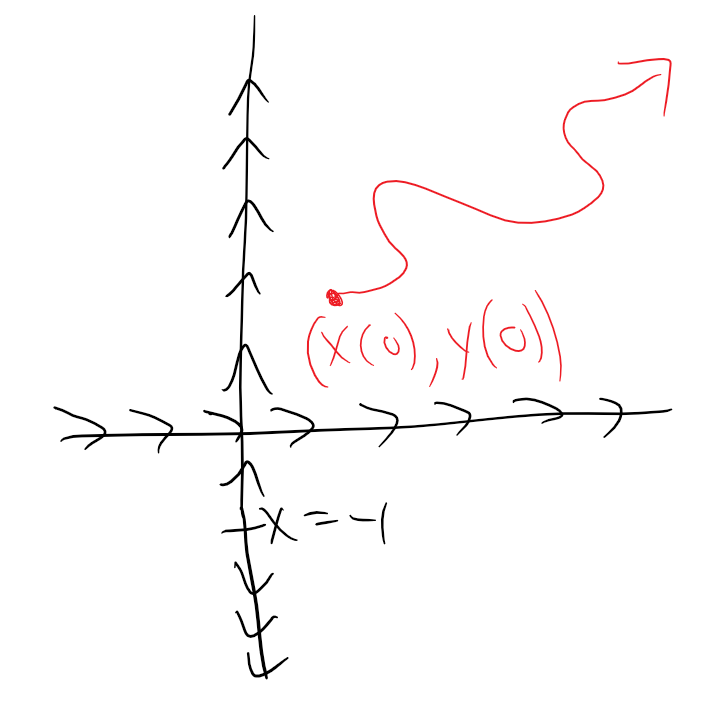
\includegraphics[width=0.6\textwidth]{Images/nullclines.png}
\end{center}

\pagebreak 

\textbf{Problem 4:} A team of ecologists contacted you to help them study the competition between two species. Based on their data, you create the following model for the populations of the two species:
\[\begin{cases}
    x' = x (3 - x -2y)\\
    y' = y(2 - x - y)
\end{cases}\]
\begin{enumerate}
    \item Find and classify the equilibrium points 
    
    Solution:
    \[\begin{cases}
        x' = 0 \implies x = 0 \,\text{ OR }\, 3 - x - 2y = 0\\
        y' = 0 \implies y = 0 \,\text{ OR }\, 2 - x- y = 0
    \end{cases}\]

    Cases:
    \[\begin{cases}
        x = 0 \implies y = 0 \, \text{ OR }\, y = 2\\
        3 - x - 2y = 0, \; y = 0 \implies x = 3\\
        \begin{cases}
            3 - x - 2y = 0\\
            2 - x - y = 0
        \end{cases} \implies 3 - x - 2y = 2 - x - y \implies y = 1, \; x = 1
    \end{cases}\]

    Equilibrium points:
    \[(0, 0), \; (0, 2), \; (3, 0), \; (1, 1)\]

    Jacobian:
    \[\nabla F(x, y) = \begin{bmatrix}
        3 - 2x - 2y & -2x\\
        -y & 2 - x - 2y
    \end{bmatrix}\]

    Classifications:
    \begin{itemize}
        \item \[\nabla F(0, 0) = \begin{bmatrix}
            3 & 0\\
            0 & 2
        \end{bmatrix} \implies \lambda = \{3, \; 2\}\]
        So (0, 0) is unstable

        \item \[\nabla F(0, 2) = \begin{bmatrix}
            -1 & 0\\
            -2 & -2
        \end{bmatrix} \implies \lambda = \{-1, \; -2\}\]
        So (0, 2) is a stable sink 

        \item \[\nabla F(3, 0) = \begin{bmatrix}
            -3 & 0\\
            0 & -1
        \end{bmatrix} \implies \lambda = \{-3, \; -1\}\]
        So (3, 0) is a stable sink

        \item \[\nabla F(1, 1) = \begin{bmatrix}
            -1 & -2\\
            -1 & -1
        \end{bmatrix} \implies (-1 - \lambda)^2 - 2 = 0\]
        \[\lambda^2 + 2\lambda - 1 = 0\]
        \[\lambda = \frac{-2 \pm \sqrt{4 - 4(-1)}}{2} = -1 \pm \sqrt{2}\]
        \[\begin{cases}
            -1 + \sqrt{3} > 0\\
            -1 - \sqrt{3} < 0
        \end{cases}\]
        So (1, 1) is a saddle
    \end{itemize}

    \item Draw a picture with the equilibrium points and their orientation (the orientation of the saddle point doesn't really matter)
    
    Solution:
    \begin{center}
        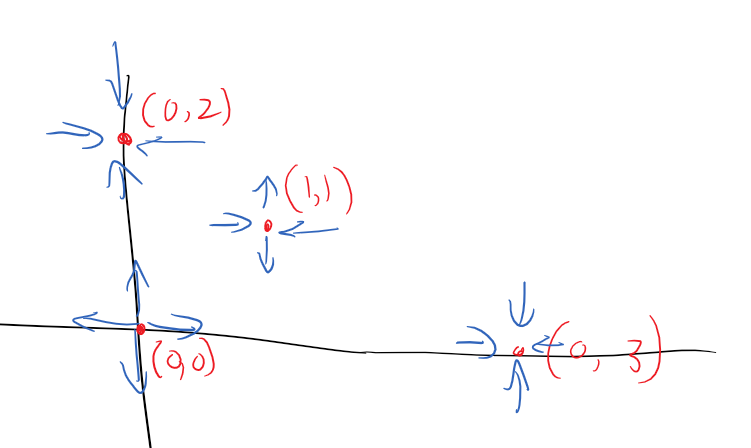
\includegraphics[width=\textwidth]{Images/equilibria.png}
    \end{center}

    \item Study the behavior of the solutions on the axes x = 0 and y = 0 and complete the orientation on the axes on your picture, like was done in lecture.
    
    \[x = 0 \implies \begin{cases}
        x' = 0\\
        y' = y (2- y)
    \end{cases}\]
    So y' is negative $(-\infty, 0)$, positive $(0, 2)$ and negative $(2, \infty)$

    \[y = 0 \implies \begin{cases}
        x' = x(3 - x)\\
        y' = 0
    \end{cases}\]
    So x' is negative for $(-\infty, 0)$, positive $(0, 3)$, and negative $(3, \infty)$

    \begin{center}
        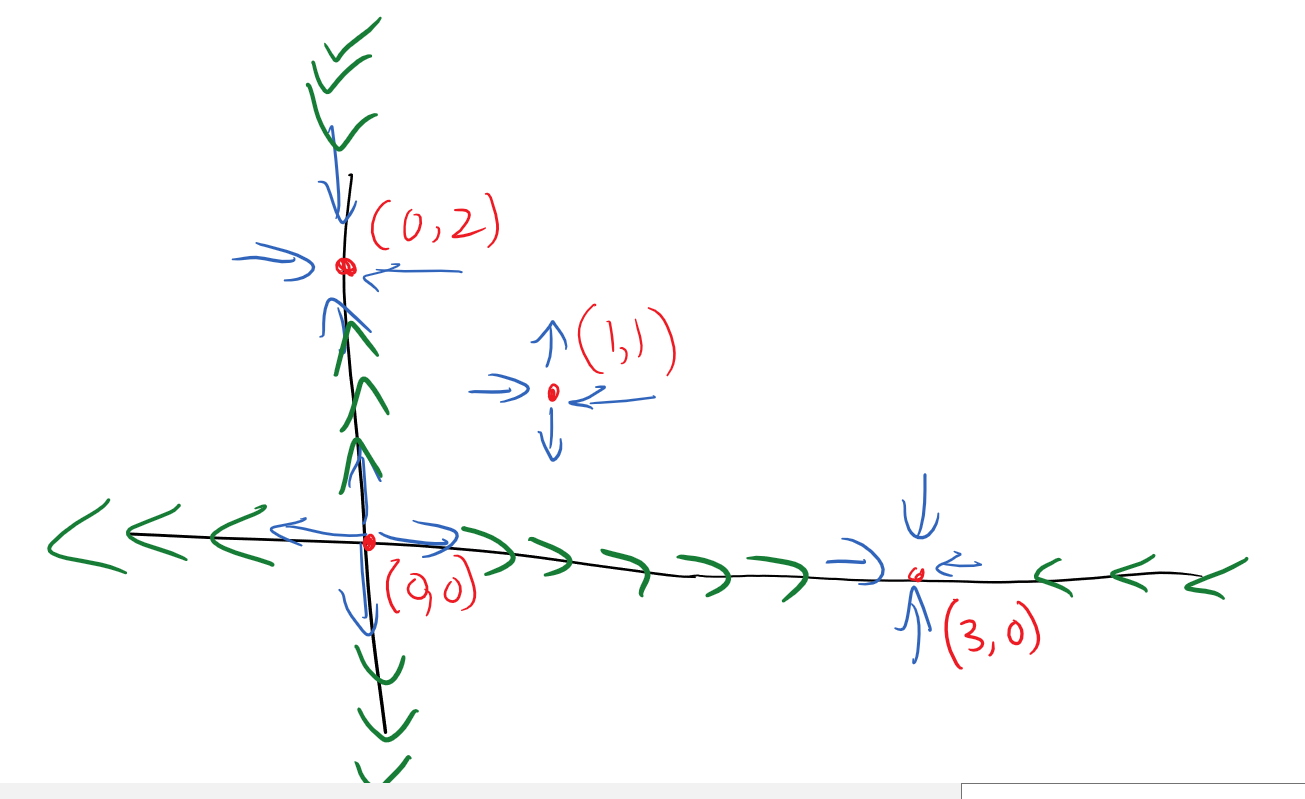
\includegraphics[width=0.9\textwidth]{Images/axes.png}
    \end{center}

    \pagebreak

    \item Draw at least 6 sample solutions on your  picture by hand. Ignore the saddle point here, it  just deflects the solutions a bit (no justification required)
     
    \begin{center}
        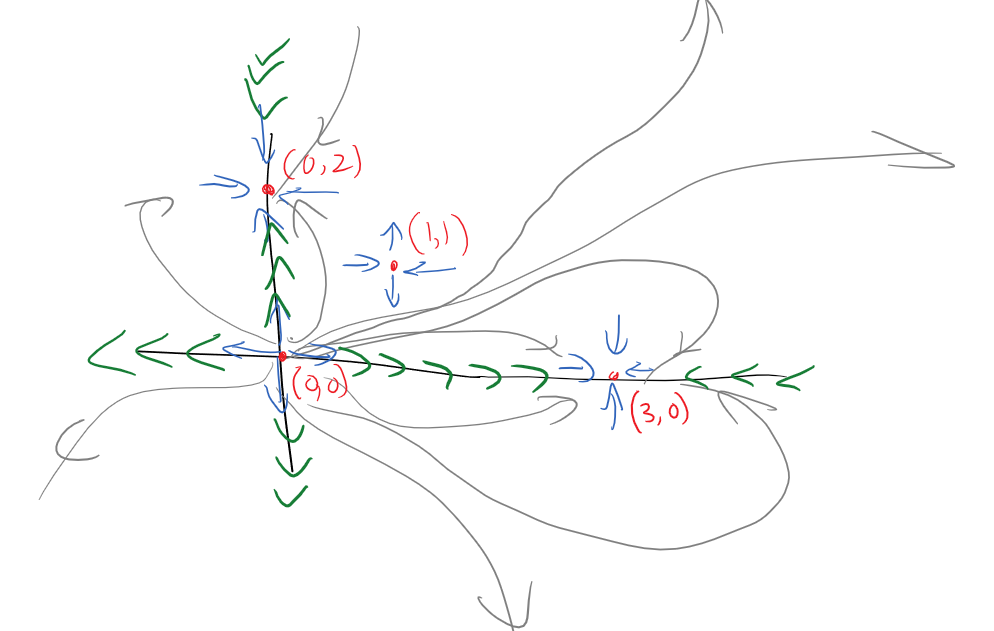
\includegraphics[width=0.8\textwidth]{Images/solutions.png}
    \end{center}

    \item Explain in your own words what happens to the populations x(t) and y(t) in the long-run (assuming both initial populations are positive) Will the populations coexist? Will both of them go extinct? Or what else?
    
    The two stable equilibria are (0, 2) and (3, 0) which suggests that one of the two -- but not both -- species will die out. 

\end{enumerate}

\end{document}